\chapter{Results and Discussion}\label{sec:resultsanddiscussion}

\subsubsection{Controlled U Gate}
\label{subsubsubsec:controlledugate}

Often there is a need for applying certain quantum gates in a controlled manner. Thus a controlled U (CU) gate is required whereby U can be any unitary single-qubit gate. The CU gate is defined as:

\begin{equation}
CU = \begin{pmatrix}
 \mathbb{1} & 0 \\ 
 0 & U
 \end{pmatrix}
\end{equation}

It is important to note that the CNOT gate is essentially a CU gate in the case of U = X. 

Most of the time the CU gate cannot be implemented directly and has to be realized through larger quantum circuits consisting of CNOT and single-qubit gates. \cite{nielsen2010quantum} describe such a decomposition as shown in Fig.~\ref{img:cudecomposition}.

\begin{figure}[ht]
   \centering
   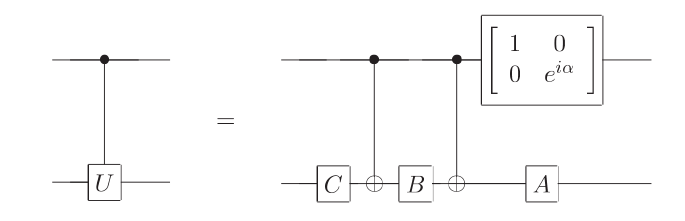
\includegraphics[width=0.7\textwidth]{img/controlledudecomp.png}
   \caption{Circuit decomposition for a controlled-U operation for single-qubit gate U.\textsuperscript{3}}
   \label{img:cudecomposition}
\end{figure}

\footnotetext[3]{Reprinted from Michael A. Nielsen and Isaac L. Chuang. Quantum Computation and Quantum Information. Cambridge University Press, 2000. Copyright 2010 by Nielsen \& Chuang.}

The idea is that when the control qubit is \0 the gate combination ABC is applied to the target qubit and has to equal the identity gate:

\begin{equation}
ABC = \mathbb{1}
\end{equation}

If and only if the control qubit is \1 then the gate sequence $e^{i\alpha}AXBXC$ is applied to the target. Since the goal is to apply the unitary U to the target qubit the following equation must be satified,

\begin{equation}
e^{i\alpha}AXBXC = U
\end{equation}

In order to find the matrices A,B,C and the additional parameter $\alpha$ the following equation has to be solved:

\begin{equation}
U = \begin{pmatrix}
 e^{i(\alpha-\frac{\beta}{2}-\frac{\delta}{2})}\cos{\frac{\gamma}{2}} & -e^{i(\alpha-\frac{\beta}{2}+\frac{\delta}{2})}\sin{\frac{\gamma}{2}} \\ 
e^{i(\alpha+\frac{\beta}{2}-\frac{\delta}{2})}\sin{\frac{\gamma}{2}} & e^{i(\alpha+\frac{\beta}{2}+\frac{\delta}{2})}\cos{\frac{\gamma}{2}}
 \end{pmatrix}
\end{equation}